In total, we did one pilot and four case studies using changes in linear and angular velocity, and oscillation angle to convey emotion. These features are depicted in Figure~\ref{fig:features}. The pilot was used to test the prototype and identify possible improvements. The values for the first two case studies were selected empirically, while for the third the Laban's description of emotion expression was followed. The final case study used values identified through the previous trials. 
%TODO add some information about the relationship among all the case studies
\begin{figure}
	\centering
	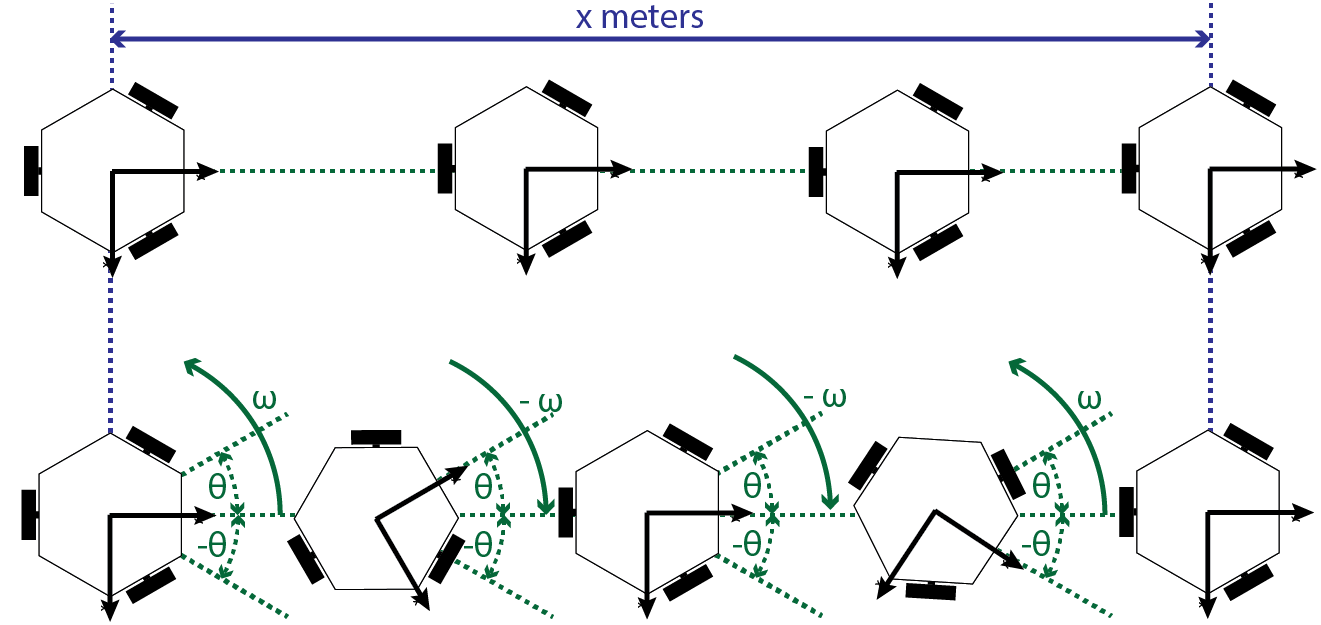
\includegraphics[width=0.75\textwidth]{./Images/ExampleMovement.png}
	\caption{Example of the features used in all case studies. $x$ represents the displacement in meters, $\omega$ is the angular velocity ($rad/s$) and $\theta$ the oscillation of the body around its center ($rad$). The upper sequence depicts a movement based only on linear velocity, while the bottom one shows a sequence with angular and linear movement.}
	\label{fig:features}
\end{figure} 
%%%%%%%%%%%%%%%%%%%%%
\section{First Case Study}
With our first version of the platform (Figure~\ref{fig:triskar-first-design}), we decided to do our first case study at the Museum of Science and Technology in Milan, where high school students and families were coming for an event that lasted 4 days. 
%%%%%%%%%%%%%%%%%%%%%%%%%
%%%%%%%%%%%%%%%%%%%%%%%%%
\subsection{Design}
Each group of participants was exposed to three rounds, in each of which the robot was performing a different emotion expression. The sequence of rounds was generated randomly without repeating any emotion in the same sequence. The subjects were asked to mark which emotion-related term that best described what they believed the robot was trying to convey, selecting among a set of nine possible options: anger, curiosity, disgust, embarrassment, fear, happiness, sadness, neutral, and pride. It was also added the option to answer: ''Unknown''. Although these ten options were enlisted, just the first eight emotions were implemented. To avoid that spectators could be influenced by previous trials, different emotions were shown to each group.\\
Additionally, it was decided to locate the robot $1.5 mts$ away from the participants and with its front facing them every time that a new emotion was showed, as shown in  Figure~\ref{fig:setup}. 
\begin{figure}
	\centering
	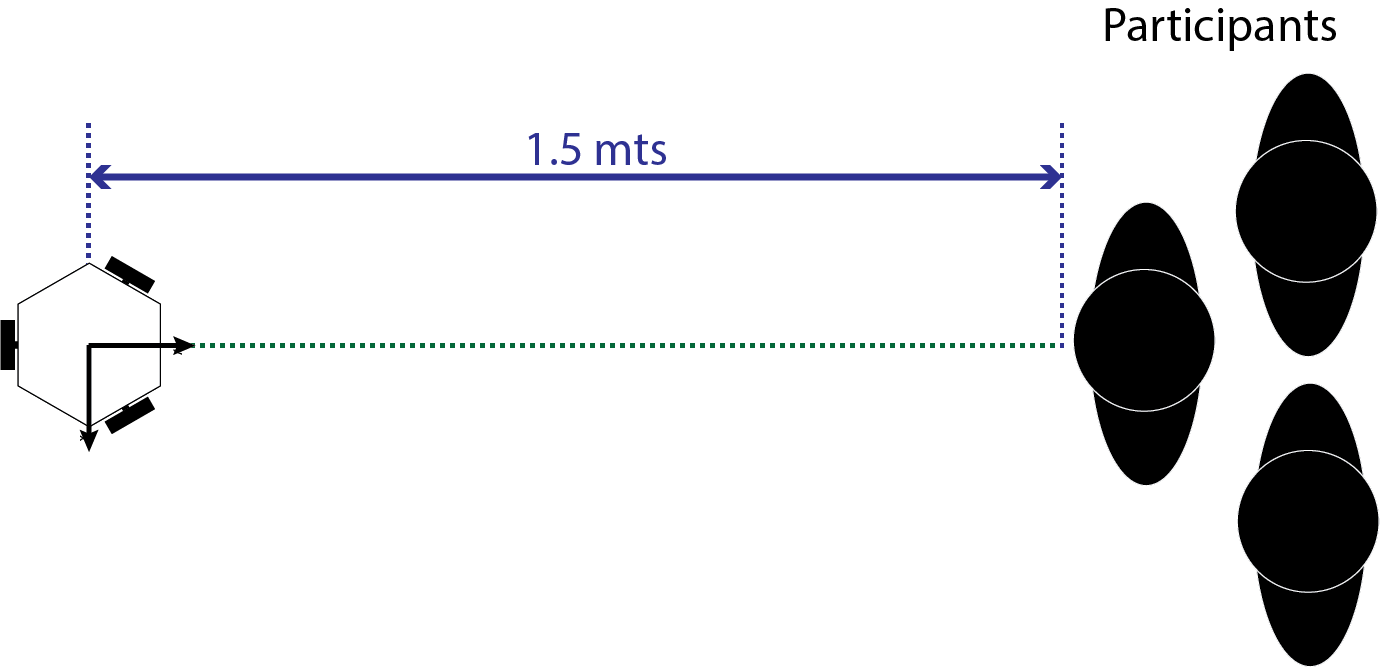
\includegraphics[width=0.7\textwidth]{./Images/FirstCase.png} 
	\caption{First case study setup.}
	\label{fig:setup}
\end{figure}  
%%%%%%%%%%%%%%%%%%%%%%%%%
%%%%%%%%%%%%%%%%%%%%%%%%%
\subsection{Emotion Description}
It was decided to follow an empirical design for this case study, consisting in taking into account the features that could be changed in the robot base and in composing them to express some basic emotions. The first implementations where tested and tuned basing on the emotions perceived by the researchers from the robot's movement.\\
The features that could easily be perceived by the observer are summarized in table~\ref{table:features}, and each selected feature is described here below:
\begin{itemize}
	\item \textit{Speed} is the target speed for the robot during the movement. It could take one out of five values: very slow (100 mm/s), slow (200 $mm/s$), normal slow (300 $mm/s$), normal (400 $mm/s$), and fast (800 $mm/s$).
	\item \textit{Front/Back} represents the fact that the robot moves backwards at some point in its movement, before going forward again; the possible values are: ''yes1``, which means that the robot goes back only once, ''yes2`` when the robot goes back twice, and ''no`` if the robot goes only forward.
	\item \textit{Shoulder} considers the movement of the upper part: ''asymmetric`` when the two beams move asymmetrically, alternatively, one forward, and the other backward, ''close``, when the upper parts get close to each other, a combination of the two (''close-2``), and ''none``. 
	\item \textit{Shoulder Amplitude} is the maximum angle that the two beams have to rotate. There are five possibilities: ''none`` ($0^\circ$), ''small`` ($10^\circ$), ''medium`` ($30^\circ$), ''large`` ($50^\circ$), and ''huge`` ($70^\circ$).
	\item \textit{Angular Velocity} $\omega$ is classified as: ''none`` (0 $mm/s$), ''slow`` (300 $mm/s$), ''medium`` (500 $mm/s$), and ''fast`` (800 $mm/s$).
	\item \textit{Body Rotation Amplitude} is the maximum  rotation angle around its center that the robot base can reach during the linear movement (it is a holonomic base); it could be: ''none`` ($0$) rad, ''small`` ($0.1$) rad, ''medium`` ($0.3$) rad, ''large`` ($0.5$) rad, and ''huge`` ($0.7$) rad.
\end{itemize}
\begin{table}[tbh]
\begin{center}
\small
\caption{Features that were presented to the audience, and their values. Embarr. is Embarrassment and Asy. is Asymmetric.}
\label{table:features}
\begin{tabular}{|p{1.5 cm}|p{1.5 cm}|c|p{1.5 cm}|p{1.6 cm}|p{1.6 cm}|m{1.5 cm}|}
\hline 
\textbf{Emotion} & \textbf{Speed} & \textbf{Front/Back} & \textbf{Shoulder} & \textbf{Shoulder Amplitude} & \textbf{Angular Velocity} & \textbf{Body Rotation Amplitude} \\ 
\hline
Anger & Fast & No & Asy. & Medium & None & Very Small \\
\hline
Sadness & Very Slow & Yes-1 & Close-2 & None & Slow & Small \\
\hline
Fear & Normal Slow & Yes-2 & Close-2 + Asy. & Small & None & None \\ 
\hline
%Fear 2 & Slow & Yes-2 & Close-2 + Asymmetric & Small & None & Small \\
%\hline
Embarr. & Slow & No & Asy. & Large & Slow & Small \\
\hline
Happiness & Fast & No & Asy. & Medium & Fast & Small \\
\hline
Disgust & Slow & No & Few Asy. & Small & None & Very Small \\
\hline
Curiosity & Normal & No & Asy. & Medium & Slow & Large \\
\hline
Neutral & Normal & No & Asy. & Medium & None & None \\
\hline
\end{tabular}
\end{center}
\vspace{-0.5cm}
\end{table} 
%%%%%%%%%%%%%%%%%%%%%%%%%
%%%%%%%%%%%%%%%%%%%%%%%%%
\subsection{Experimental Setup}
There was no specific group size, since this was determined by the amount of people that got close to the booth at a given moment. Therefore, there were groups with just one person and others with 24 persons. The total amount of volunteers was 154: 55 males, 26 females, and 73 that did not specify their gender. The average age was 21.95 with a standard deviation of 12.26, minimum age was 5, maximum 62.
\subsection{Results}
Table~\ref{table:results_1} shows the results obtained in the first case study. 
\begin{table}[tbh]
\caption{Answers obtained the first case study. On each row is the emotion that was intended to express, and on the columns the reported emotions.
.}
\small
\label{table:results_1}
\centering
\begin{tabular}{|c|c|c|c|c|c|c|c|c|c|c|c|c|}
\hline
\backslashbox{Presented}{Reported} & 
\rotatebox{90}{\textbf{Anger}}&
\rotatebox{90}{\textbf{Curiosity}}&
\rotatebox{90}{\textbf{Disgust}}&
\rotatebox{90}{\textbf{Embarr.}}&
\rotatebox{90}{\textbf{Fear}}&
\rotatebox{90}{\textbf{Happiness}}&
\rotatebox{90}{\textbf{Neutral}}&
\rotatebox{90}{\textbf{Pride}}&
\rotatebox{90}{\textbf{Sadness}}&
\rotatebox{90}{\textbf{Unk.}}&
\rotatebox{90}{\textbf{Tot.}}&
\rotatebox{90}{\textbf{Percentage}}\\
\hline
Anger &23 &11 &3 &4 &7 &6 &1 &0 &0 &4 &59&38.98\%\\
\hline
Curiosity &2 &9 &3 &9 &2 &3 &2 &8 &3 &0 &41&21.95\%\\
\hline
Disgust& 1 & 11& 1& 3& 7& 3& 6& 8& 5& 1& 46&2.17\%\\
\hline
Embarr. & 3& 11& 0& 8& 9& 3& 0& 4& 2& 1& 41&19.51\%\\
\hline
Fear & 3& 29& 5& 25& 22& 2& 2& 0& 2& 2& 92&22.82\%\\
\hline
Happiness & 15& 4& 0& 2& 3& 28& 4& 4& 2& 1& 63&44.44\%\\
\hline
Neutral & 5& 0& 1& 1& 0& 1& 0& 3& 2& 0& 13&0\%\\
\hline
Sadness & 4& 5& 1& 11& 13& 0& 2& 3& 7& 0& 46&23.81\%\\
\hline
\end{tabular}
\end{table}
Table~\ref{table:results_1} shows that the best emotion perceived was Happiness and the worst one Disgust, with 44\% and 2\% respectively of accuracy. Moreover, some movements were designed to convey a specific emotion, but a different emotion was perceived. For example the intended Sadness was identified by 14\% of subjects exposed to it, while 25.5\% perceived it as Fear. The neutral behaviour was not much considered, possibly because people, in this setting, expected to see something specific, not a neutral movement. To analyse whether each emotional expression was misinterpreted with others a Fisher's exact test was applied for each possible combination of emotions implemented. Additionally, a Holm-Bonferroni correction was applied for multiple comparisons to get better p-value estimation. 
The results showed that people perceived the following implementations as similar, having a $p-value>0.05$: curiosity-disgust, curiosity-embarrassment, curiosity-sadness, disgust-embarrassment, disgust-sadness, embarrassment-fear, embarrassment-sadness, and fear-sadness. 

Moreover, an analysis was done per groups, for each presented emotion. Excluding unknown and uncertain answers, we have considered the answers of each subject that was presented an emotion produced by the robot. For each emotion we considered how many subjects in each group recognized it, how many identified a different emotion, how many identified the considered emotion when presented another one (in any of the other two experiences each did), and how many recognized an emotion different from the considered one when presented a different emotion. This lead for each presented emotion to a table like the one reported in Table~\ref{table:singleEmotion} for Happiness. 
\begin{table}
\begin{center}
\small
\caption{Example of table compiled for each emotion on the subjects that have been presented each emotion (here Happiness).}
\label{table:singleEmotion}
\begin{tabular}{|c|c|c|}
\hline 
\backslashbox{Presented}{Reported}&Happiness&Other\\
\hline 
Happiness&28&4\\
\hline 
Other&30&96\\
\hline
\end{tabular}
\end{center}
%\vspace{-0.5cm}
\end{table}
For each of these tables the classification accuracy and the no-information rate (NIR), i.e. the accuracy that had been obtained by random selection, have been computed with the R package CARET~\cite{caret}.
The results show that some implementations of emotion expression (i.e., Anger ($p-value=1e-3$) and Happiness ($p-value=2.8e-5$)) have been recognized by the respective panels, while others are not.
%%%%%%%%%%%%%%%%%%%%%
\section{Second Case Study}
Since the results of the first case study showed that the recognition of most of the designed emotions was still quite poor, it was decided to try again with the same emotions, but this time a context to the emotional state of the robot was provided by playing a little scene. This is motivated by the fact that that emotions are triggered by stimuli~\cite{Plutchik2001,cacioppo2000handbook}.
%%%%%%%%%%%%%%%%%%%%%%%%%
%%%%%%%%%%%%%%%%%%%%%%%%%
\subsection{Design}
A little scene was created for each emotion to give a context to the participants. The procedure and questionnaire were the same as the one adopted for the first case. However, it was added a variant of the Fear emotion (Fear2), in which the robot finishes its trajectory far from the person. As done in the first case, each group was exposed to three emotions and the sequence presented to each group was different to eliminate the chance to influence other groups. The sequences were generated randomly and without repeating an emotion in a sequence.\\
As in the first case study, the total distance covered by the robot was $1.5 mts$, but this time the robot was facing the actor. The distance from the participants to the robot and actor was $1.5 mts$, as shown in Figure~\ref{fig:setup2}. 
\begin{figure}
	\centering
	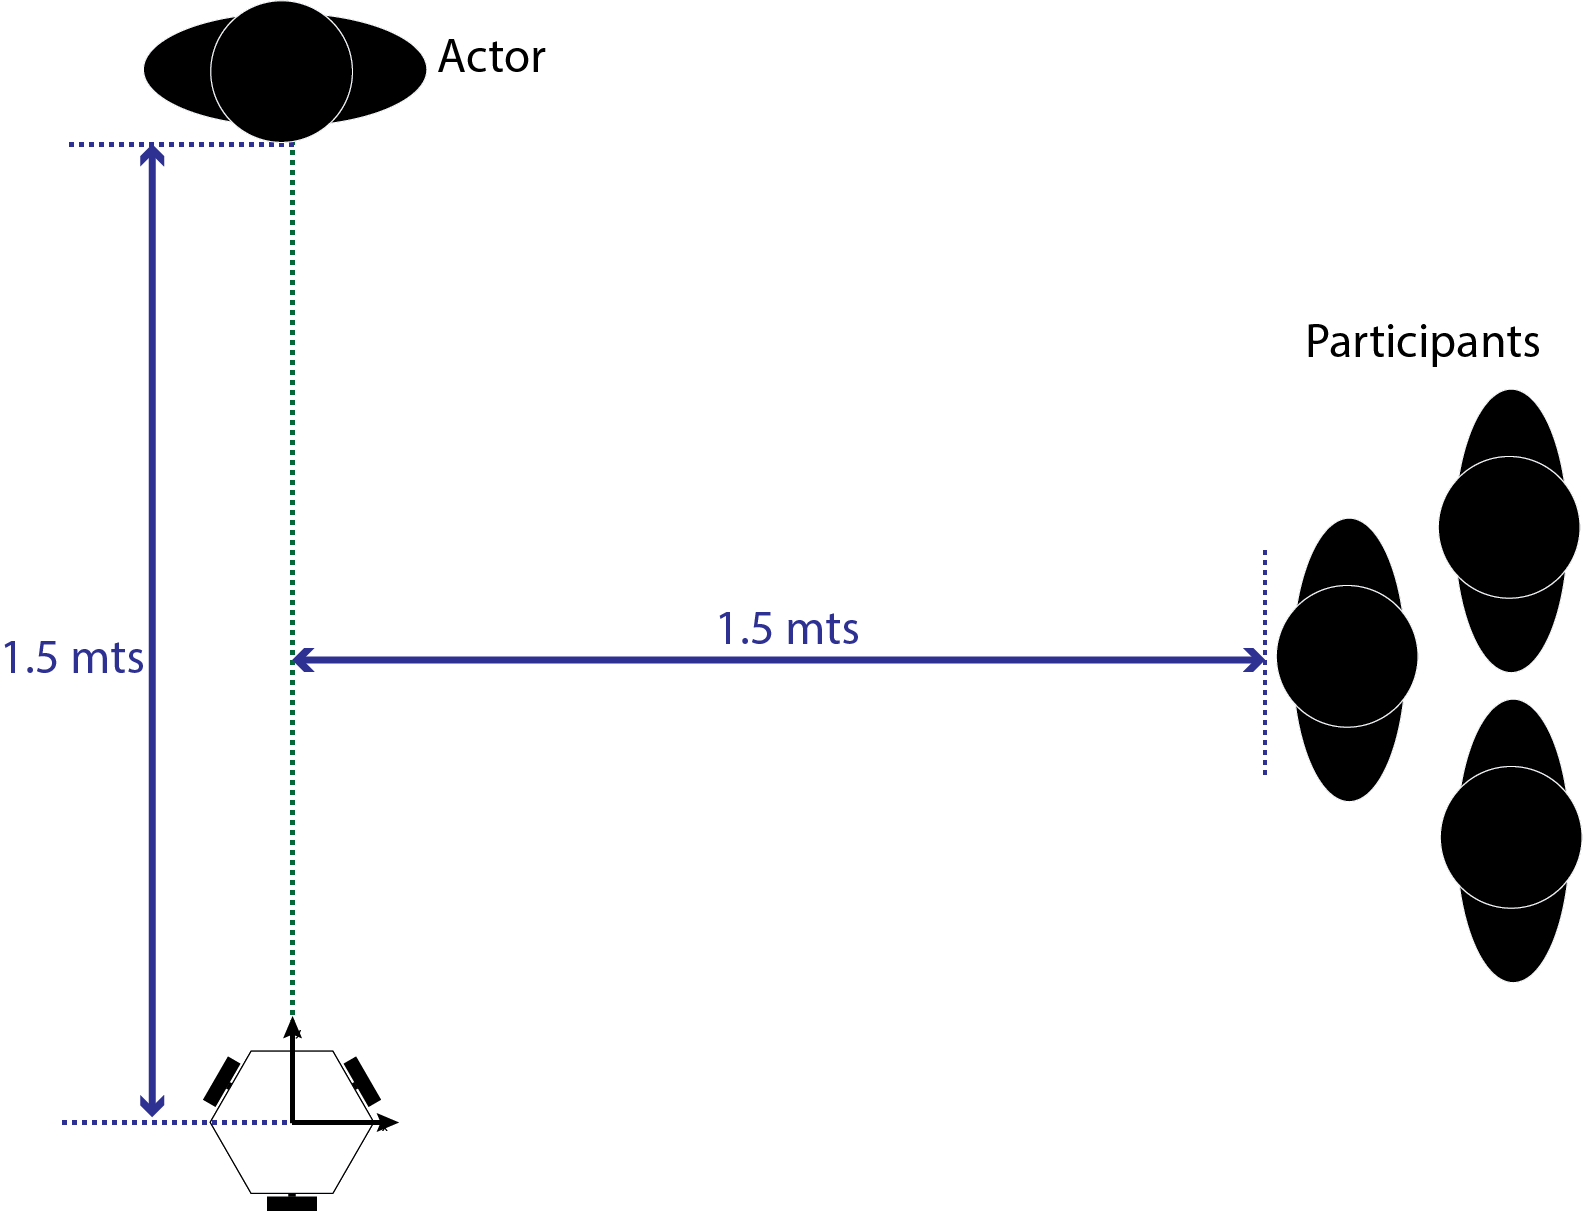
\includegraphics[width=0.6\textwidth]{./Images/SecondCase.png} 
	\caption{Setup of the second case study.}
	\label{fig:setup2}
\end{figure}
%%%%%%%%%%%%%%%%%%%%%%%%%
%%%%%%%%%%%%%%%%%%%%%%%%%
\subsection{Study}
The laboratory open day of 2013 was used to perform the scenes and actions and to collect data. Eight groups participated, each one with approximately 20 volunteers for a total of 156: 51 males, 17 females, and 88 that did not provide their gender. The average age was 26.34 with a standard deviation of 12.44, and with a minimum age of 11 and maximum of 65.
%%%%%%%%%%%%%%%%%%%%%%%%%
%%%%%%%%%%%%%%%%%%%%%%%%%
\subsection{Results}
Table~\ref{table:results_2} shows the results obtained in the second case study.
\begin{table}[tbh]
\caption{Answers obtained in the second case studies. On each row is the emotion that was intended to express, and on the columns the reported emotions.}
\small
\label{table:results_2}
\centering
\begin{tabular}{|c|c|c|c|c|c|c|c|c|c|c|c|c|}
\hline
\backslashbox{Presented}{Reported} & 
\rotatebox{90}{\textbf{Anger}}&
\rotatebox{90}{\textbf{Curiosity}}&
\rotatebox{90}{\textbf{Disgust}}&
\rotatebox{90}{\textbf{Embarr.}}&
\rotatebox{90}{\textbf{Fear}}&
\rotatebox{90}{\textbf{Happiness}}&
\rotatebox{90}{\textbf{Neutral}}&
\rotatebox{90}{\textbf{Pride}}&
\rotatebox{90}{\textbf{Sadness}}&
\rotatebox{90}{\textbf{Unk.}}&
\rotatebox{90}{\textbf{Tot.}}&
\rotatebox{90}{\textbf{Percentage}}\\
\hline
Anger &41 &1 &2 &0 &6 &9 &0 &2 &0 &1 &62&66.13\%\\
\hline
Curiosity &8 &38 &0 &3 &0 &4 &1 &1 &1 &4 &60&63.33\%\\
\hline
Disgust& 6& 2& 5& 4& 3& 0& 4& 7& 4& 3& 38&13.16\%\\
\hline
Embarr. & 7& 2& 1& 4& 12& 0& 0& 1& 10& 0& 37&10.81\%\\
\hline
Fear & 0& 13& 0& 17& 10& 6& 0& 0& 0& 0& 46&21.74\%\\
\hline
Fear2 & 3& 0& 5& 5& 35& 0& 1& 0& 2& 0& 51&68.63\%\\
\hline
Happiness & 0& 1& 0& 0& 5& 55& 1& 0& 0& 1& 63&87.30\%\\
\hline
Neutral & 1& 3& 2& 5& 7& 9& 5& 5& 1& 1& 39&12.82\%\\
\hline
Sadness & 0& 4& 2& 22& 14& 0& 2& 3& 15& 1& 63&23.81\%\\
\hline
\end{tabular}
\end{table}
In the second case study, the results were considerably better, where four out of the nine showed emotions had a percentage of recognition higher than 60\% (Anger, Happiness, Curiosity and Fear2). Another important point to highlight is that Sadness, Fear and Embarrassment were still perceived as different emotions. As it was done for the first case study, a Fisher's exact test and Holm-Bonferroni correction were applied for each possible combination of implemented emotions. The results suggest that no implementation was considered as similar to others by the participants, since for all we have $p-value<\alpha$.  Comparing the percentage from both cases, it is possible to see that giving information about the context that produces the current emotional state of the robot improves its recognition. However, if the conveyed emotion does not match the scene, the audience does not recognize it. This shows that even giving information about the situation, and using a human actor to provide the context, people could not recognize the emotion if the correct features are not exploited. To verify this, it was done a comparison between the results obtained for each emotion in both cases doing a Fisher's exact test. The results suggest that implementations of Disgust ($p=0.088$), Fear ($p=0.206$) and Sadness ($p=0.269$) are perceived as the same in both cases. This would suggest that the combination of stimuli (scene + actor) and correct robot's movements are necessary to the correct emotional interpretation. However with the adopted setup, it was impossible to determine which factor had more relevance.
%%%%%%%%%%%%%%%%%%%%%
\section{Third Case Study}
The third case study was designed to explore the possibility to adopt for robot's movements the emotional movement descriptions reported in human body studies, and followed the methodology used by Sharma and collaborators~\cite{Sharma2013} to select the emotions to be implemented and enlisted in the questionnaire. The second version of the platform was used in this case study (Figure~\ref{fig:triskar-second-design}).
%%%%%%%%%%%%%%%%%%%%%%%%%
%%%%%%%%%%%%%%%%%%%%%%%%%
\subsection{Experimental setup}
From the previous experience it was decided to implemented just four emotions, which reduce the number of possible sequences. To select the emotions to be implemented, the \textit{circumplex model of affect} was adopted, as it was suggested by Sharma. The emotions implemented were: \textit{Happiness} (I quadrant), \textit{Anger} (II quadrant), \textit{Sadness} (III quadrant), and \textit{Content} (IV quadrant). To reduce the probability that the correct emotion could be selected by chance four additional emotions were selected following the same selection procedure of the implemented ones, one from each quadrant. These emotions were: \textit{Frustration}, \textit{Boredom}, \textit{Astonishment} and \textit{Tiredness}. The final questionnaire had nine possibilities (eight emotions and ``Unknown''). 

In order to study the influence that could be generated by the given list of emotions to the participants, it was used an open questionnaire that did not list any emotion, but rather had a space where participants could write a term to answer the question: "\textit{What emotion the robot has expressed?}".
The setup used in this case study is depicted in the Figure~\ref{fig:setup2}.
\begin{figure}
	\centering
	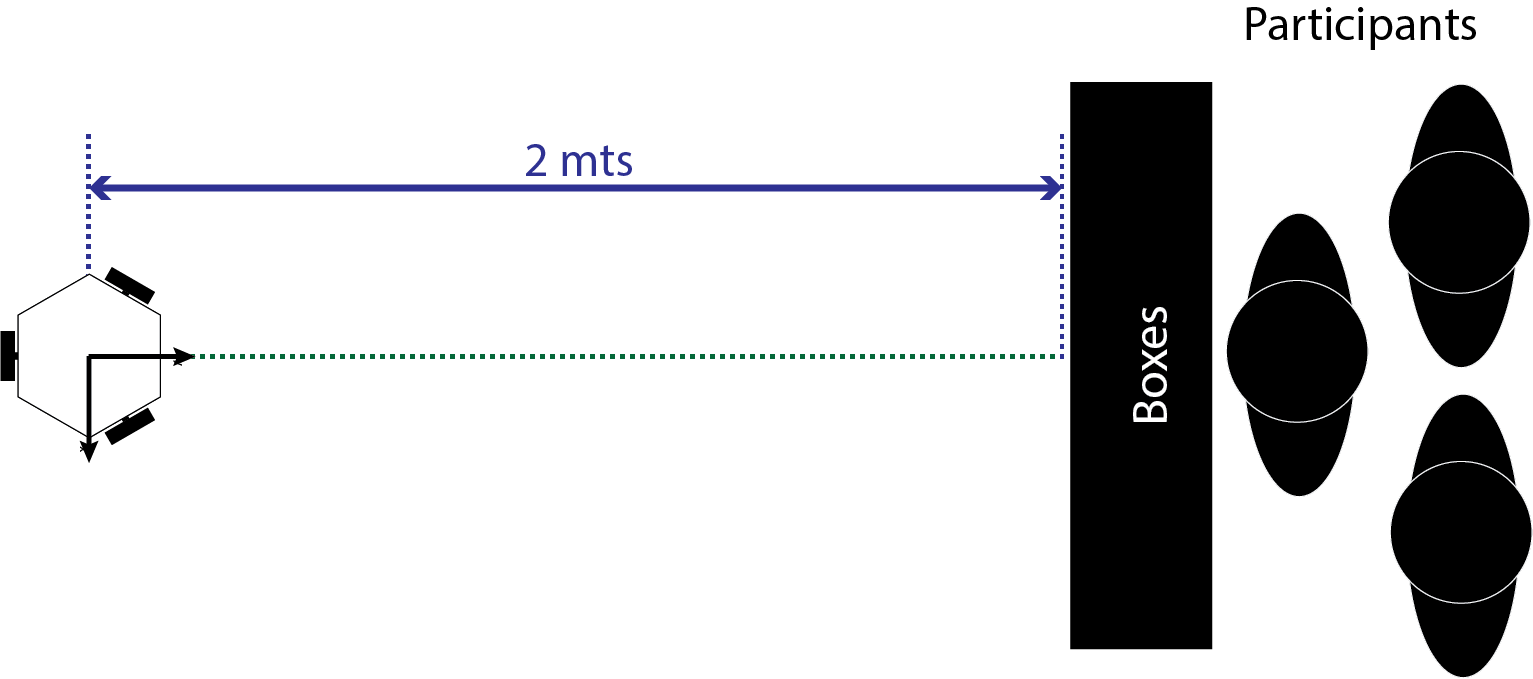
\includegraphics[width=0.6\textwidth]{./Images/ThirdCase.png} 
	\caption{Setup of the third case study.}
	\label{fig:setup2} %TODO check whether it is the correct setup. Yes, it was two meters and with some boxes to not let the participants move over the robots path. OK, just because the number did not match (setup2 for the 3rd case study)
\end{figure}
%%%%%%%%%%%%%%%%%%%%%%%%%
%%%%%%%%%%%%%%%%%%%%%%%%%
\subsection{Emotion Descriptions} 
Due to the scarce literature about emotional parameters in robotics, the selection of the parameters for the implemented emotions were made following the literature in human emotion projection~\cite{Nadia2013, Crane2013}.
Generally speaking, these works use the Laban's notation to code their findings, which leaves to the designer (and the reader) their specific interpretation.\\
The specific values selected for each emotion are reported as follow:
\begin{itemize}
	\item \textit{\textit{Anger}:} the strong force required by Laban was interpreted as a high speed and then a sudden drop, thus it was decided to have a velocity of $500mm/sec$ for $50mm$ and then a velocity of $300mm/sec$. An oscillation during the whole trajectory was also added; that was between [0.086, -0.086] radians with an angular velocity of $3.5 rad/sec$.
	\item \textit{\textit{Happiness}:} as in \textit{Anger}, for the first $50mm$ the velocity was $500mm/sec$, then it went down to $400mm/sec$ for another $50mm$, and then up again to $800mm/sec$ for the rest of the movement. 
	An oscillation between [0.26, -0.26] radians with an angular velocity of $3rad/sec$ was also added.
	\item \textit{Sadness:} the required "low energy" was interpreted as low speed and then slowing down the pace, thus a velocity of $150mm/sec$ was used for the first $200mm$, a velocity $250mm/sec$ for the next $200mm$, and for the rest a velocity of $300mm/sec$. This emotion expression did not include any angular rotation.
	\item \textit{Content:} the velocity was $150mm/sec$ for the first $200mm$, then $300mm/sec$ for the rest. The maximum and minimum angle of oscillation were [0.175, -0.175] with angular velocity of $0.17rad/sec$
\end{itemize}
It is important to notice that these parameters do not include any changes in the upper part of the body, since the changes done in the platform significantly decreased the emotion expression of the upper part.
%%%%%%%%%%%%%%%%%%%%%%%%%
%%%%%%%%%%%%%%%%%%%%%%%%%
\subsection{Study}
This case study was done during the Rome Maker Faire, 2014. During a period of four days, people were asked to participate to this study. Each subject was exposed to two rounds: in each one, the robot was performing a different emotion. During the first two days, the open questionnaire was used, while during the last two days the multiple option questionnaire was used. The total number of volunteers for the closed list questionnaire was 91: 52 males, 38 females, and 11 that chose not to specify their gender. The average age was 30.98 years, with standard deviation of 15.12, minimum age was 4 and maximum 71. The total amount of participants assessing the study with the open questionnaire was 84: 47 males, 36 females, and 1 that did not specify; the average age was 24 years, with standard deviation of 15.8, minimum age was 5 and maximum 59. 
%%%%%%%%%%%%%%%%%%%%%%%%%
%%%%%%%%%%%%%%%%%%%%%%%%%
\subsection{Results}
From the open questionnaire, different terms to describe both emotions and mental states were obtained. In table~\ref{table:open_questionnaire} are reported the results. In order to reduce the quantity of words, words that have a similar meaning were grouped, for example words as \textit{Fear}, \textit{Terror}, \textit{Scared}, and \textit{Worried} were grouped under the label \textit{Fear}. Also, three out of four emotions (\textit{Anger}, \textit{Happiness} and \textit{Sadness}) were at least once listed correctly. \textit{Sadness} and \textit{Content} were mostly perceived as \textit{Fear}, being written 31\% and 28\% of the time for each of these two emotions respectively.\\
From these results is possible to highlight two important facts:
\begin{itemize}
	\item The language richness to refer to emotions and the vague definition of emotions let people to use words that could not be directly associated to a specific emotion. 
	\item The movements that could be designed as emotional are also associated to mental states of the robots. This is evident in the words obtained from the presentation of four ''emotional'' movements, such as \textit{cold} (referring that the robot was feeling cold), \textit{tenderness}, \textit{shyness}, \textit{power}, \textit{hurry}, \textit{looking for something}, \textit{he wants something}, \textit{enthusiasm}, \textit{sympathy}, \textit{vanity}, and \textit{obedience}. 
\end{itemize}
%%%%%%%%%%%%%%%%%%%%%%%%%%%
\begin{table}
\centering
		\caption{Results obtained from the open questionnaire.}
		\label{table:open_questionnaire}
		\small
			\begin{tabular}{|c|c|c|c|c|c|}
				\hline
					\backslashbox{Presented}{Reported}&\textit{Anger}&\textit{Happiness}&\textit{Sadness}&\textit{Content}&Total\\
				\hline
					\textit{Anger}& 3&6&7&5&21\\
				\hline
					\textit{Happiness}&12& 18&0&6&36\\
				\hline
					\textit{Sadness}&0&0& 8&3&11\\
				\hline
					\textit{Content}&2&0&0& 0&2\\
				\hline
					\textit{Fear}&4&5&14&13&36\\
				\hline
					\textit{Tiredness}&1&0&1&1&3\\
				\hline
					\textit{Cold}&2&0&2&1&5\\
				\hline
					\textit{Shyness}&1&0&4&4&9\\
				\hline
					\textit{Agitated}&4&1&0&0&5\\
				\hline
					\textit{Power}&4&1&0&0&5\\
				\hline
					\textit{Hurry}&0&1&0&0&1\\
				\hline
					\textit{Looking for something}&1&0&1&0&2\\
				\hline
					\textit{He wants something}&1&0&1&0&2\\
				\hline
					\textit{Tenderness}&1&0&1&2&4\\
				\hline
					\textit{Uncertainty}&1&2&0&0&3\\
				\hline
					\textit{Enthusiasm}&1&0&0&0&1\\
				\hline
					\textit{Sympathy}&1&0&2&4&7\\
				\hline
					\textit{Curiosity}&1&2&3&3&9\\
				\hline
					\textit{Shame}&0&0&0&1&1\\
				\hline
					\textit{Nothing}&1&2&1&0&4\\
				\hline
					\textit{Vanity}&1&0&0&0&1\\
				\hline
					\textit{Obedience}&0&0&0&1&1\\
				\hline
					\textit{Total}&43&38&44&46&171\\
				\hline
			\end{tabular}
\end{table}
A summary of the obtained answers is provided in Table~\ref{table:result_list_emotions}.
\begin{table}
\centering
\small
\caption{Answers obtained in the case study.}
		\label{table:result_list_emotions}
		\begin{tabular}{|c|c|c|c|c|c|c|c|c|c|c|}
			\hline	
\rotatebox{90}{\backslashbox{Presented}{Reported}}&
\rotatebox{90}{\textit{Anger}}&
\rotatebox{90}{ \textit{Happiness}} &
\rotatebox{90}{\textit{Sadness}}&
\rotatebox{90}{\textit{Content}}&
\rotatebox{90}{\textit{Frustration}}&
\rotatebox{90}{\textit{Boredom}}&
\rotatebox{90}{\textit{Astonishment}}&
\rotatebox{90}{\textit{Tiredness}}&
\rotatebox{90}{\textit{Unknown}}&
\rotatebox{90}{Total}\\	
			\hline
				\textit{Anger}& 19&8&1&5&7&2&5&1&0&48\\
			\hline
				\textit{Happiness}&18& 19&0&9&5&1&5&1&0&58\\
			\hline
				\textit{Sadness}&1&9& 12&2&4&5&7&6&0&46\\
			\hline
				\textit{Content}&2&8&7& 4&6&8&5&10&0&50\\	
			\hline	
			\end{tabular}
\end{table}
An analysis was done for each emotion, therefore it was created a contingency matrix such as it was done in the first case study.
Additional two confusion matrices were created: one merging the results from all high (\textit{Anger}, \textit{Happiness}, \textit{Frustration} and \textit{Astonishment}) and low (\textit{Sadness}, \textit{Content}, \textit{Boredom}, and \textit{Tiredness}) arousal emotions; and the other one merges the results of positive (\textit{Happiness}, \textit{Content}, \textit{Astonishment}, and \textit{Tiredness}) and negative (\textit{Anger}, \textit{Frustration}, \textit{Boredom}, and \textit{Sadness}) emotions. For each of these tables were calculated the positive predictive value, accuracy and a Pearson's $\chi^2$. The results are shown in table~\ref{table:Precision}. They show that there is significant evidence to conclude that anger, happiness, and sadness have an impact in the perception of the emotion, while the implementation of content does not have any significant impact in the emotion perception. Moreover, high and low arousal are perceived as different, but this is not the case for positive and negative valence. \\
%%%%%%%%%%%%%%%%%%%%%%%%%%%%%%%%%%%
\begin{table}
	\begin{center}
\small
		\caption{Accuracy, precision and results of Pearson's $\chi^2$ for each contingency matrix with $\alpha = 0.05$ for the third case study.} 
\label{table:Precision}
		\begin{tabular}{|p{3 cm}|p{2 cm}|c|c|c|}
		\hline
		\textbf{Presented Emotion} & \textbf{Positive Predicted Value} & \textbf{Accuracy} & \textbf{$\chi^2(1)$} & \textbf{p-value}\\
		\hline		
		High/Low Arousal & 0.81 & 0.69 & 28.7 & 8.29e-8\\
		\hline
		Positive/Negative Valence & 0.56 & 0.55 & 1.9 & 0.167\\
		\hline
		\hline
		Anger & 0.4 & 0.75&13.923 & 1.9e-4\\
		\hline
		Happiness & 0.33 & 0.68&4.88&2.7e-2\\
		\hline
		Sadness & 0.26 & 0.79&15.22&9.5e-5\\
		\hline
		Content & 0.08 & 0.69&6e-2&0.8 \\		 
		\hline
		\end{tabular}
	\end{center}
\end{table}
To analyse whether each emotion expression was misinterpreted with other implementations, a Fisher's exact test and Holm-Bonferroni correction were applied for each possible combination of emotions implemented, which gives a total of seven combinations. %The results are shown in the the Table~\ref{table:chi}. 
The results suggest that the implementations of anger and happiness ($p-value=0.492$), and, respectively, sadness and content ($p-value=0.492$) are interpreted as similar, while the other emotion expressions are distinguished from each other.\\ %TODO The same p-value? Very strange...

%%%%%%%%%%%%%%%%%%%%%%%%%%%%%%%%%%%
%\begin{table}
%\small
%	\begin{center}
%		\caption{Pairwise comparison among all the implemented emotions using Fisher's exact test for both questionnaires with $\alpha = 0.05$ for the third case study. The * indicates that the p-value was adjusted using the Holm-Bonferroni correction for multiple comparisons.} 
%		\label{table:chi}
%		\begin{tabular}{|c|c|c|c|c|}
%		\hline
%		\multirow{2}{*}{\textbf{Pair Compared}}&\multicolumn{2}{|c|}{\textbf{List Questionnaire}}&\multicolumn{2}{|c|}{\textbf{Open Questionnaire}}\\
%		\cline{2-5}
%		& \textbf{p-value} & \textbf{p-value*}& \textbf{p-value} & \textbf{p-value*}\\
%		\hline
%		Anger vs Happiness & 0.4903&0.9&0.2879&0.492\\
%		\hline 
%		Anger vs Sadness  & 2.85e-5&1.01e-5&6.09e-7&3.05e-6\\
%		\hline
%		Anger vs Content &1.2e-4&9e-5&7.9e-3&0.0239\\
%		\hline
%		Happiness vs Sadness &7.81e-7&6e-7&1.8e-8&1.08e-7\\
%		\hline
%		Happiness vs Content &2.2e-6&6e-7&3.4e-4&1.36e-3\\
%		\hline
%		Sadness vs Content& 0.7036&0.9&0.246&0.492\\
%		\hline		
%		\end{tabular}
%	\end{center}
%\end{table}
From the results of both questionnaires, we can say that \textit{Anger} and \textit{Happiness} were confused, as well \textit{Sadness} and \textit{Content}. \textit{Fear} was written as emotion when the two emotions with low arousal (\textit{Sadness} and \textit{Content}) were shown. These results show that velocity plays a role to elicit emotions, but that it is necessary to add additional features (e.g., changes on body shape) to increase the discrimination among low and high arousal emotions.
%%%%%%%%%%%%%%%%%%%%%%
\section{Fourth Case Study}
After the first and third case studies, it was evident the necessity to better understand how the characteristics are related with each other and how they can be used to convey emotions. Therefore, it was decided to perform an experiment to get a better insight on the contribution of angular and linear velocity, angle of oscillation, direction and orientation. To cross-validate the data collected in this experiment, we decided to do a final case study.
%%%%%%%%%%%%%%%%%%%%%%%%%
%%%%%%%%%%%%%%%%%%%%%%%%%
\subsection{Experimental setup}
From the results obtained on our experiments, we selected two combinations (angular velocity, oscillation angle, linear velocity, orientation and direction) with the higher Krippendorff's alpha coefficient~\cite{Klaus2007} and mean for each emotion studied in a experiment done after third case study. As in the previous case studies, a questionnaire was used. However, this time the emotions selected were the same used during the experiment: anger, fear, sadness and happiness. Moreover, two mental states were added: excited and tender, which corresponds to high and low arousal, respectively. As it was done in the previous cases, the questionnaire included the option ''unknown''. Although the platform used was the last version (Figure~\ref{fig:triskar-third-design}), the upper part was cut off to allow comparisons with the platform used in the other experiments. The case study set up could be seen in the Figure~\ref{fig:setup_fourth}.
\begin{figure}
	\centering
	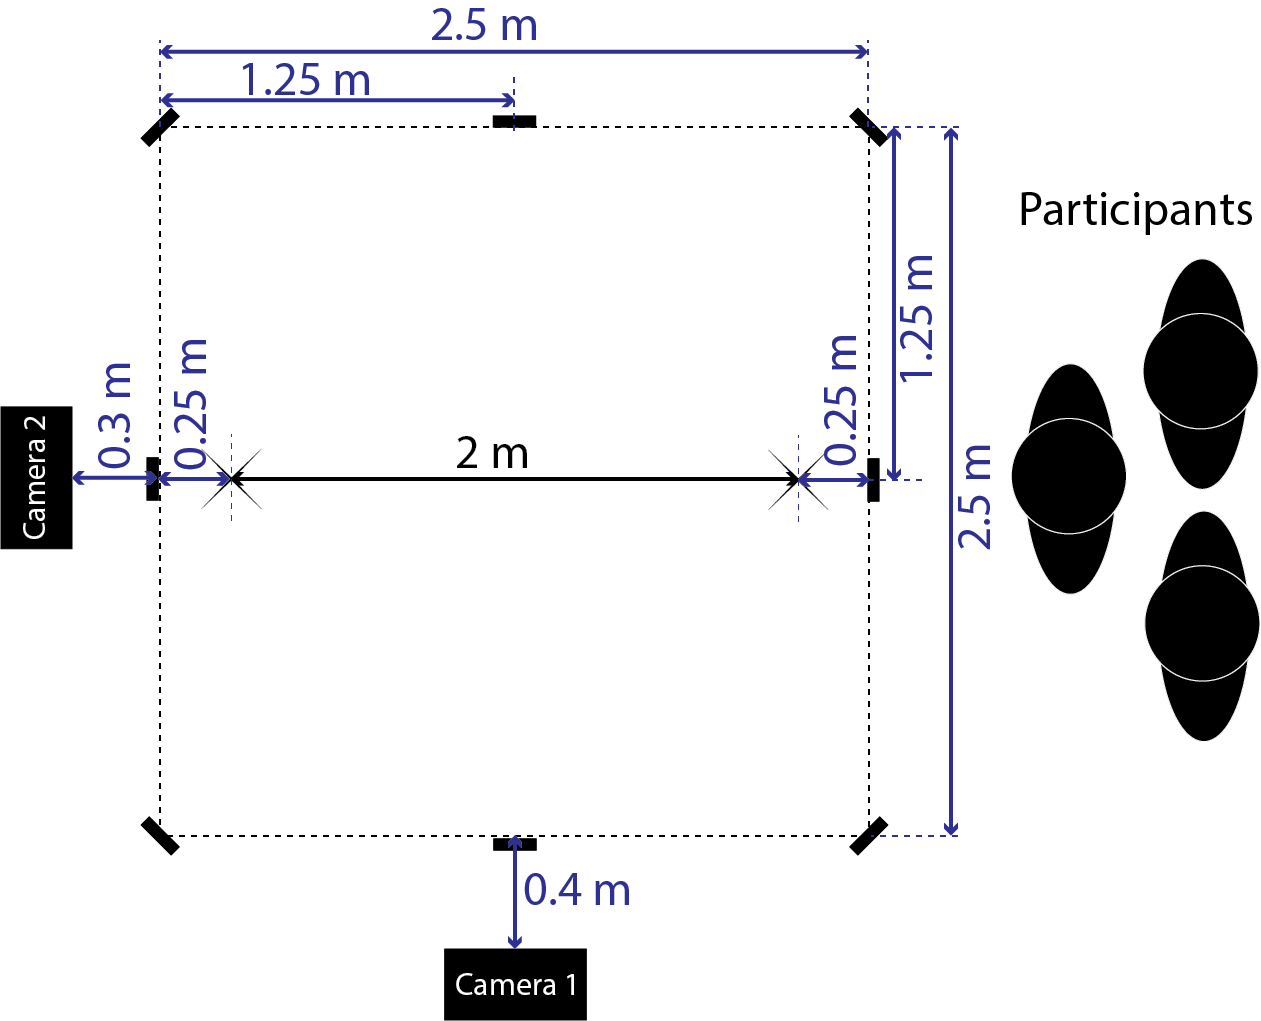
\includegraphics[width=0.60\textwidth]{./Images/FourthCase.png} 
	\caption{Environment setup for the fourth case study. The crosses symbolize the two possible starting points.}
	\label{fig:setup_fourth}
\end{figure} 
%%%%%%%%%%%%%%%%%%%%%%%%%
%%%%%%%%%%%%%%%%%%%%%%%%%
\subsection{Emotion Descriptions} 
The selected emotion descriptions could be seen in Table~\ref{table:features_2}
\begin{table}[tbh]
\begin{center}
\caption{Combination of features selected for the fourth case study.}
\label{table:features_2}
\small
\begin{tabular}{|c|c|p{2.5 cm}|p{2 cm}|p{2 cm}|p{2.5cm}|}
\hline 
\textbf{Emotion} & \textbf{Direction} & \textbf{Orientation} & \textbf{Linear Velocity} $mm/sec$& \textbf{Angular Velocity} $rad/sec$& \textbf{Oscillation Angle} $rad$\\
\hline
Happiness 1 & Getting close & Looking at the person & $500$  & $3$ & $0.349$ \\
\hline
Happiness 2 & Getting close & Looking at the person & $900$ & $3$ & $0.174$ \\
\hline
Fear 1 & Getting far & Looking at the person & $900$ & $2$ & $0.174$ \\
\hline
Fear 2 & Getting far & Looking at the person & $500$ & $2$ & $0.087$ \\
\hline
Angry 1 & Getting far & Giving the back & $500$ & $3$ & $0.087$ \\
\hline
Angry 2 & Getting close & Looking at the person & $900$ & $1$ & $0.087$ \\
\hline
Sadness 1 & Getting far & Giving the back & $200$ & $1$ & $0.349$ \\
\hline
Sadness 2 & Getting close & Giving the back & $200$ & $1$  & $0.349$ \\
\hline
\end{tabular}
\end{center}
\end{table} 
%%%%%%%%%%%%%%%%%%%%%%%%%
%%%%%%%%%%%%%%%%%%%%%%%%%
\subsection{Study}
This case study was done during the 2015 Researchers' Night. During a period of two days, people were asked to participate to this study. As in the third case study, each participant was exposed to only two emotions. The emotion sequences presented to the participants were established before hand, and randomized. The total number of participants was 256: 128 males, 126 females, and 2 unknown. The average age was 27.29 years, with standard deviation of 16.5, minimum age was 4 and maximum 76. 
%%%%%%%%%%%%%%%%%%%%%%%%%
%%%%%%%%%%%%%%%%%%%%%%%%%
\subsection{Results}
Table~\ref{table:result_fourth} summarizes the results obtained during the case study.
\begin{table}
\centering
\small
\caption{Summary of the answers obtained in the fourth case study.}
		\label{table:result_fourth}
		\begin{tabular}{|c|c|c|c|c|c|c|c|c|c|}
			\hline	
\rotatebox{90}{\textbf{Presented/Reported } }&
\rotatebox{90}{\textbf{Happiness}}&
\rotatebox{90}{ \textbf{Anger}} &
\rotatebox{90}{\textbf{Fear}}&
\rotatebox{90}{\textbf{Sadness}}&
\rotatebox{90}{\textbf{Excitement}}&
\rotatebox{90}{\textbf{Tenderness}}&
\rotatebox{90}{\textbf{Other}}&
\rotatebox{90}{\textbf{Total}}&
\rotatebox{90}{\textbf{Percentage}}\\	
			\hline
			Happiness 1&8&16&7&4&16&4&7&62&13\%\\
			\hline
			Happiness 2&11&11&6&2&19&3&1&53&21\%\\
			\hline
			Anger 1&7&5&6&2&21&7&1&49&10\%\\
			\hline
			Anger 2&14&29&13&2&13&3&2&76&38\%\\
			\hline
			Fear 1&6&2&28&1&9&6&0&52&54\%\\
			\hline
			Fear 2&7&3&37&2&20&4&1&74&50\%\\
			\hline
			Sadness 1&3&5&17&14&5&16&5&65&22\%\\
			\hline
			Sadness 2&5&5&15&28&6&15&7&81&35\%\\
			\hline
			\end{tabular}
\end{table} 
It could be observed that both implementations of Happiness are confused with Anger and Excitement, as it could have been expected. The first implementation of Anger was mostly confused with Excitement, which was perceived by twenty one over forty nine participants, while the second implementation showed an improvement from 10\% to 38\% on recognition. This implementation was perceived also has Happiness, Fear and Excitement by fourteen, twelve, and thirteen respectively. Both implementations of Fear have a high level of recognition 54\% and 50\% and mostly confused with excitement, nine for the first implementation and twenty for the second implementation. Lastly, the first implementation of Sadness was confused with Fear and Tenderness by twelve and sixteen respectively. The second implementation was confused again with Fear and Tenderness by thirteen and twenty-eight respectively.\\
To verify these misinterpretations among the implemented emotions, a Fisher's exact test and Holm-Bonferroni correction were applied for 10 different combinations. The results are shown in Table~\ref{table:result_compare_fourth}. As the results suggest, the implementation of Anger is the only one that was considered as different.\\
\begin{table}
\centering
\small
\caption{Pairwise comparison among all the implemented emotions using Fisher's exact test for both questionnaires with $\alpha = 0.05$ for the fourth case study. The * indicates that the p-value was adjusted using the Holm-Bonferroni correction for multiple comparisons.}
		\label{table:result_compare_fourth}
		\begin{tabular}{|c|c|c|}
			\hline	
\textbf{Pair Compared} & \textbf{p-value} & \textbf{p-value*}\\	
			\hline
			Happiness 1 vs Happiness 2 &0.38&1.0\\
			\hline
			Anger 1 vs Anger 2 & 7.3e-4&4.4e-3\\
			\hline
			Anger 2 vs Happiness 1 & 0.137&0.69\\
			\hline
			Anger 2 vs Happiness 2 & 0.157&0.69\\
			\hline
			Fear 1 vs Fear 2 & 0.74&1.0\\
			\hline
			Sadness 1 vs Sadness 2 & 0.665&1.0\\
			\hline
			Fear 1 vs Sadness 1& 8.35e-5&5.8e-4\\
			\hline
			Fear 1 vs Sadness 2 & 5e-7&4e-6\\
			\hline
			Fear 2 vs Sadness 1 & 2e-7&1.8e-6\\
			\hline
			Fear 2 vs Sadness 2 & 1e-7&1e-6\\
			\hline
			\end{tabular}
\end{table} 
As it was done in the previous case studies a contingency matrix was computed.
For each of these tables were calculated the positive predictive value, accuracy and a Pearson's $\chi^2$. The results are shown in table~\ref{table:Precision2}. They show that there is significant evidence to conclude that one implementation of Anger, and both those of Fear and Sadness have an impact in the perception of the emotion, while both implementations of Happiness and one of Anger do not have any significant impact on the emotion perception.\\
\clearpage
\begin{table}
\centering
\small
\caption{Accuracy, precision and results of Pearson's $\chi^2$ for each contingency matrix with $\alpha = 0.05$ for the fourth case study.} 
\label{table:Precision2}
		\begin{tabular}{|p{3 cm}|p{2 cm}|c|c|c|}
		\hline
		\textbf{Presented Emotion} & \textbf{Positive Predicted Value} & \textbf{Accuracy} & \textbf{$\chi^2(1)$} & \textbf{p-value}\\
		\hline
		Happiness 1 & 0.13 & 0.79 & 0.11 & 0.74\\
		\hline
		Happiness 2 & 0.21 & 0.81& 3.7 &0.054\\
		\hline
		Anger 1 & 0.1 & 0.8 & 3.8e-29 & 1\\
		\hline
		Anger 2 & 0.38 & 0.81 & 34.4 & 4.47e-9\\
		\hline
		Fear 1 & 0.54 & 0.8 & 36.2 & 1.8-e9\\
		\hline 
		Fear 2 & 0.5 & 0.78 & 35.8 & 5.3e-10\\
		\hline
		Sadness 1 & 0.22 & 0.85 & 27.4 & 1.63e-7\\
		\hline
		Sadness 2 & 0.35 & 0.85 & 72.9 & 2.2e-16\\		 
		\hline
			\end{tabular}
\end{table} 
It is important to notice that the results were obtained using the lower part of the robot without any change in shape. Another factor to consider is the high impact of the words enlisted in the questionnaire had in the detection rate. These words included two mental states that could be confused with the other four emotions enlisted, as it is reflected in the results. Despite the bias generated by these two words, the recognition rates of five over eight emotion expressions were over 35\%, being the two implementations of Fear the ones with the highest recognition rate (54\% for the first and 50\% for the second).